\section{Parser Generator}

In this section, we introduce a way to automatically generate JavaScript parsers
from given ECMAScript specifications. First, we explain \( \bnfes \), an extension
of Backus-Naur form(BNF) used in ECMAScript to describe lexical and
syntactic grammars of JavaScript. We propose a recursive descent parser generator
that both supports backtracking and lookahead tokens to correctly support
\( \bnfes \) notations. We implement our idea by extending Scala parser combinators.
The implementation also supports the automatic semicolon insertion,
one of the most distinctive parsing features in ECMAScript.

\subsection{\( \bnfes \): Grammars for ECMAScripts}

Backus-Naur form(BNF) is proposed to represent context-free grammars(CFGs).
ECMAScript provides their lexical and syntactic grammars using \( \bnfes \),
an extension of BNF for ECMAScript.
It consists of a number of \textit{productions} with the following forms:
\[
  \NT{A}(\param_1, \cdots, \param_k) ::=
  (\cond_1 \Rightarrow)^? \rhs_1 \mid
  \cdots \mid
  (\cond_n \Rightarrow)^? \rhs_n
\]
The left-hand side represents a parametric non-terminal \( \NT{A} \) with
multiple boolean parameters \( \param_1, \cdots, \param_n \).
If a non-terminal takes no parameters, parenthesis are omitted for the brevity.
A production has multiple right-hand sides with optional conditions.
A condition \( \cond \) is either a boolean parameter \( \param \)
or its negation \( ! \param \).
For example, consider the following production:
\[
  \NT{A}(\param) ::= \param \Rightarrow \T{a}
  \mid \; !\param \Rightarrow \T{b}
  \mid  \T{c}
\]
Then, \( \NT{A}(\kwt) \) means \( \T{a} \mid \T{c} \)
and \( \NT{A}(\kwf) \) means \( \T{b} \mid \T{c} \).

Each right-hand side \( \rhs \) is a sequence of the following symbols:
\begin{itemize}
  \item \( \boxed{\epsilon} \): empty sequence
  \item \( \boxed{\T{a}} \): terminal symbols
  \item \( \boxed{\NT{A}(\argument_1, \cdots, \argument_k)} \): non-terminal symbols
  \item \( \boxed{\symb?} \): optional symbols
  \item \( \boxed{\pm \symb} \): positive/negative lookahead symbols
  \item \( \boxed{\symb \butnot \symb'} \): exclusive symbols
  \item \( \boxed{\nolt} \): no line-terminator symbols
\end{itemize}

The empty sequence \( \epsilon \) passes without any conditions
and a terminal symbol is any token.
A non-terminal symbol \( \NT{A}(\argument_1, \cdots, \argument_k) \)
takes multiple arguments and each of them \( \argument_i \) is
a boolean value \( \kwt \), \( \kwf \) or a parameter \( \param_i \).
An optional symbol \( \symb? \) is same with \( \symb \mid \epsilon \).
A positive(negative) lookahead symbol \( +\symb \)(\( -\symb \))
checks that the symbol \( \symb \) succeeds(fails) and
\textit{never consumes any input}.
The exclusive symbols \( \symb \butnot \symb' \)
first checks that the symbol \( \symb \) succeeds
and then checks that the parsing result does not correspond to \( \symb' \).
The no-line terminal symbol \( \nolt \) is a special symbol
that restricts the white spaces between two other symbols.

\subsection{Lookahead Parsers}

Our goal is to automatically generate JavaScript parsers from ECMAScript
grammars written in \( \bnfes \). There are several options for parser generators;
ANTLR, Lex/Yacc, Bison, and PEG. Among them, we decided to use
Scala parser combinators defined under \textit{parsing expression grammars(PEG)}.
PEG follows top-down (LL-style) parsing approaches and there are two different
categories; predictive parser and recursive descent with backtracking.
Predictive parsers are widely used in general and LL(k) parsers are typical
examples of predictive top-down parsers.
They choose a right-hand sides based on predicting the next tokens in deterministic
manners. In the other hand, PEG is a recursive descent parser with
\textit{backtracking}. It visits each right-hand side in order and backtrack
into the previous rules when parsing fails.
Thus, it is possible to use each production itself as a parser
in PEG. Moreover, There are several reasons why we extend Scala parser combinator
to deal with ECMAScript lexers and grammars written in \( \bnfes \):

\begin{itemize}
  \item \textbf{Context-Sensitive Tokens} ECMAScript tokens are context-sensitive
    because of the JavaScript regular expressions and template strings.
    For example, the code \( \code{/x/g} \) might be a single regular expression token
    or four tokens that represent division by variables \( \code{x} \) and \( \code{g} \)
    depending on enclosing contexts. Thus, lexers should be evaluated during the parser
    not before the parser. Scala parser combinators also treat lexers as parsers thus
    it is possible to use appropriate lexers depending on the parsing contexts.
  \item \textbf{\( \bnfes \) Symbols} PEG is suitable grammars to represent
    \( \bnfes \) symbols. We will explain detailed conversion from
    \( \bnfes \) grammars into Scala parser combinators in section~\ref{sec:convert-bnfes}.
  \item \textbf{Multiple Starting Non-terminals} After ECMAScript 6, grammars support
    both scripts and modules as starting point of parsers. In Scala parser combinators,
    it is possible to parse input string using any non-terminals as parsers.
  \item \textbf{Parsing in Run-time} JavaScript supports \( \code{eval} \)
    function that parses given JavaScript String values into codes and evaluates them.
    Moreover, there is special phrases ``the \( N \) that is \textit{covered by}
    \( P \)'' in syntax-directed abstract algorithms.
    It means that the syntax tree \( P \) is parsed with generalized parsers because
    it needs evaluation contexts to correctly choose specific parsers.
    When the interpreter meets the above phrase, the specific parsers are now
    decided into \( N \) thus we should parse again the given syntax tree \( P \) with
    the non-terminal \( N \) in run time.
\end{itemize}

\subsubsection{Prioritized choices}
However, unfortunately, there is fundamental problem in PEG-based parsers;
\textit{prioritized choices}.
In PEG, the pipe operator ( \( \mid \) ) denotes a prioritized choice,
unlike CFG that deals with it in non-deterministic manners.
It means that PEG always pick the first success right-hand side even though
there exist other success choices in remaining right-hand sides.
While ECMAScript grammars are deterministic languages, some non-terminals
accepts multiple right-hand sides for a given input strings.
It distort the meaning of ECMAScript grammars.
For example, consider the following simplified grammars for JavaScript expressions:
\[
  \begin{array}{r@{~}c@{~}l}
    \NT{A} &::=& \NT{T} \T{;} \mid \NT{A} \; \T{+} \; \NT{T} \T{;} \\
    \NT{T} &::=& \T{a} \mid \T{a} \T{(} \T{b} \T{)}\\
  \end{array}
\]
While it represents deterministic grammar, the non-terminal \( \NT{T} \)
should accept both right-hand sides if the given string is \( \code{a(b);} \).
However, PEG-based parser fails to parse it
because the first right-hand side \( \T{a} \) is always tried
first in the non-terminal \( \NT{T} \).
Thus, the latter one \( \T{a} \T{(} \T{b} \T{)} \) is not reachable in PEG.
A simple solution is to change the order of right-hand sides;
\( \NT{T} ::= \T{a} \T{(} \T{b} \T{)} \mid \T{a} \).
However, it is not easy to ensure which order is correct
because their inclusion relationship should be calculated.
Moreover, some productions are not possible to resolve them
by simply re-ordering right-hand sides:
\[
  \begin{array}{r@{~}c@{~}l}
    \NT{A} &::=& \NT{B} \; \T{b}\\
    \NT{B} &::=& \T{a} \mid \T{a} \; \T{b}\\
  \end{array}
\]
The non-terminal \( \NT{A} \) should successfully parse two strings \( \code{ab} \)
and \( \code{abb} \). However, the non-terminal \( \NT{A} \) accepts only
\( \code{ab} \) and it accepts only \( \code{abb} \) when \( \NT{B} \) has
reversed order. It means that we should re-structure
the above rules to accept both strings in traditional PEG grammars.

\subsubsection{Lookahead tokens}
To alleviate such problems, we propose \textit{lookahead parsers},
which is extended recursive descent parsers with backtracking and
\textit{lookahead tokens}.
It keeps track of the next possible tokens using statically
calculated first tokens of each symbols using algorithm in
Figure~\ref{fig:first-tokens}. For example, the following steps explain
how to utilize lookahead tokens during parsing processes with
the input \( \code{a(b);} \):

\begin{figure}
\centering
\[
  \begin{array}{l@{~}c@{~}l}
    \rhsfirst{\symb_1 \cdots \symb_n} &=& \symbfirst{\symb_1} \firstplus
    \symbfirst{\symb_2 \cdots \symb_n}\\
    && \text{where} \; x \firstplus y = \left\{
    \begin{array}{ll}
      x \cup y & \text{if} \; \emptyfirst \in x\\
      x & \text{otherwise}\\
    \end{array}
    \right.\\
    \symbfirst{\epsilon} &=& \{ \emptyfirst \}\\
    \symbfirst{\T{a}} &=& \{ \T{a} \} \\
    \symbfirst{\NT{A}(\argument_1, \cdots, \argument_k)} &=&
    \rhsfirst{\rhs_1} \cup \cdots \cup \rhsfirst{\rhs_n}\\
    && \text{where} \; \NT{A}(\argument_1, \cdots, \argument_k) =
    \rhs_1 \mid \cdots \mid \rhs_n\\
    \symbfirst{\symb?} &=& \symbfirst{\symb} \cup \{ \emptyfirst \}\\
    \symbfirst{+\symb} &=& \symbfirst{\symb}\\
    \symbfirst{-\symb} &=& \{ \emptyfirst \}\\
    \symbfirst{\symb \butnot \symb'} &=& \symbfirst{\symb}\\
    \symbfirst{\nolt} &=& \{ \emptyfirst \}\\
  \end{array}
\]
\caption{Over-approximated first tokens of \( \bnfes \) symbols}
\label{fig:first-tokens}
\end{figure}

\Tree[.\(\NT{A}[\emptyfirst]\)
[.\(\NT{T}\T{;}[\emptyfirst]\)
[.\(\NT{T}[\T{;}]\)
\sout{\(\T{a}[\T{;}]\)}
[.\(\T{a}\T{(}\T{b}\T{)}[\T{;}]\)
[.\(\T{a}[\T{(}]\) \(\boxed{\T{a}}\) ]
[.\(\T{(}\T{b}\T{)}[\T{;}]\)
[.\(\T{(}[\T{b}]\) \(\boxed{\T{(}}\) ]
[.\(\T{b}\T{)}[\T{;}]\)
[.\(\T{b}[\T{)}]\) \(\boxed{\T{b}}\) ]
[.\(\T{b}\T{)}[\T{;}]\)
[.\(\T{)}[\T{;}]\) \(\boxed{\T{)}}\) ] ] ] ] ] ]
[.\(\T{;}[\emptyfirst]\)
\(\boxed{\T{;}}\) ] ] ]

Each node \( \symb^*[\la] \) denotes a sequence of symbols \( \symb^* \) with
lookahead tokens \( \la \), which is the set of tokens.
The parsing process follows pre-order traversals.
It starts from the starting non-terminal \( \NT{A} \) with the special
lookahead \( \emptyfirst \), which denotes the end of inputs.
Then, it visits the first right-hand side \( \NT{T} \T{;} \) with the same lookahead.
Each symbol will be visited with the corresponding lookahead, that is the
first tokens of the right next symbol.
For example, for the symbol \( \NT{T} \), the next symbol is \( \T{;} \)
and its first token is itself. Thus, the parser visits \( \NT{T} \)
with the lookahead \( \T{;} \). The most important point in this parsing process
is the first right hand side \( \T{a} \) of the non-terminal \( \NT{T} \).
It is visited with the lookahead \( \T{;} \) but the next token of the input string
\( \code{a(b);} \) is \( \code{(} \) not \( \code{;} \).
Thus, it fails to parse the input string even though the current token is
same with the terminal \( \T{a} \).
Thus, the parser could visit the next right-hand side \( \T{a}\T{(}\T{b}\T{)} \)
and finally the input \( \code{a(b);} \) is successfully parsed.

We formally define semantics of lookahead parsers
in Figure~\ref{fig:laparser} by converting them into the given parsers.
The helper function \( \getlap{\la} \) generates a parser by combining all
tokens in the lookahead \( \la \) using prioritized choices.
In this case, the order does not change the semantics of lookahead parsers
because \( \getlap{\la} \) just check whether it contains the given token or not.

\begin{figure}
\centering
\[
  \begin{array}{l@{~}c@{~}l}
    (\symb_1 \cdots \symb_n)[\la] &=&
    \symb_1[\symbfirst{\symb_2 \cdots \symb_n} \firstplus \la] \;
    (\symb_1 \cdots \symb_n)[\la]\\
    \epsilon[\la] &=& +\getlap{\la}\\
    \T{a}[\la] &=& \T{a} \; +\getlap{\la} \\
    \NT{A}(\argument_1, \cdots, \argument_k)[\la] &=&
    \rhs_1[\la] \mid \cdots \mid \rhs_n[\la]\\
    && \text{where} \; \NT{A}(\argument_1, \cdots, \argument_k) =
    \rhs_1 \mid \cdots \mid \rhs_n\\

    \symb?[\la] &=& \symb[\la] \mid \epsilon[\la]\\
    (\pm\symb)[\la] &=& \pm(\symb[\la]) \\
    (\symb \butnot \symb')[\la] &=& \symb[\la] \butnot \symb'\\
    \nolt &=& \nolt \; +\getlap{\la}\\
  \end{array}
\]
\caption{Formal semantics of lookahead parsers}
\label{fig:laparser}
\end{figure}

\subsection{Implementation}

We implement lookahead parsers by extending Scala parser combinators.
We define \( \code{LAparser} \) trait to represent lookahead parser
and it has two members; first tokens and a function from lookahead tokens into parsers
described in Figure~\ref{fig:first-tokens} and Figure~\ref{fig:laparser}, respectively.
There exists two different issues in implementing the lookahead parsers in Scala
to treat ECMAScript syntax written in \( \bnfes \).

\paragraph{Performances} One of critical weak points of recursive descent parsing
with backtracking is its performance. Basically, it needs exponential time related
to the input size because of the backtracking mechanism. Fortunately,
Ford et al~\cite{packrat} proposed Packrat parsing that provides linear
time complexity based on memoization technique. The main idea is that it treats
each parser as a function from the current input position into the parsing result.
Thus, it just memoizes each parser based on input positions. It dramatically reduces
the redundant parsing trials. In a similar way, we treat each lookahead parser as
a function from a pair of lookahead tokens and input positions into parsing results.

\paragraph{Left Recursions} The other issue is that recursive descent parsers
does not support left recursions in grammars. If a grammar has left recursions,
the parser falls into an infinite loop. To resolve this problem,
Warth et al~\cite{packrat-lr} proposed a way to support not only direct left
recursions but also indirect ones in Packrat parsing.
The basic idea is extends the memoization technique to support grow the parsing
results. We believe that it is conceptually possible to support direct and indirect
left recursions by applying the Warth's approach.
\inred{However, fortunately, it is not necessary to handle indirect left
recursions in order to deal with ECMAScript syntax because the all
versions of ECMAScript only have direct left recursions.}
Thus, we decided to just remove direct left recursions by defining sub productions
and carefully build the abstract syntax trees.

\begin{figure}
  \centering
  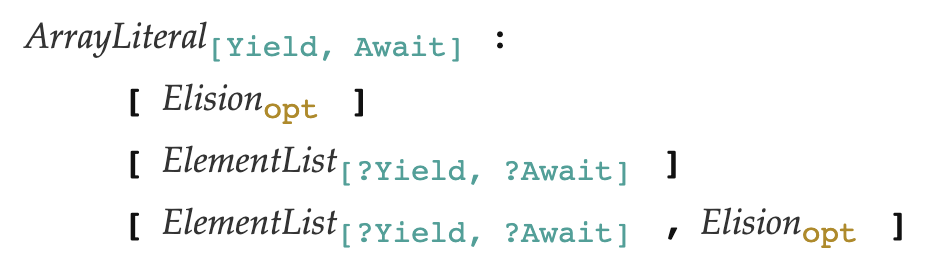
\includegraphics[height=6em]{img/array_literal.png}
  \[
    \begin{array}{l}
      \NT{ArrayLiteral}(Yield, Await) ::=\\
      \qquad \T{[} \; Elision? \; \T{]}\\
      \qquad \T{[} \; ElementList(Yield, Await) \; \T{]}\\
      \qquad \T{[} \; ElementList(Yield, Await) \; \T{,} Elision? \; \T{]}\\
    \end{array}
  \]
  \caption{Array literals defined in ES2019 and its \( \bnfes \)}
  \label{fig:array-literal}
\end{figure}

\subsubsection{AST generations}
We first automatically generate abstract syntax tree(AST) as Scala case classes
from the given \( \bnfes \) grammar that represents a version of ECMAScript.
For lexical grammars, their structures are not used in ECMAScript semantics
thus we gives them String types. For parser grammars, we need to
automatically synthesize a Scala file that has classes of syntax trees.
For each production \(
  \NT{A}(\param_1, \cdots, \param_k) ::=
  (\cond_1 \Rightarrow)^? \rhs_1 \mid
  \cdots \mid
  (\cond_n \Rightarrow)^? \rhs_n
\), the AST generator defines the \( \code{A} \) trait and
multiple sub classes \( \code{Ai} \) of \( \code{A} \) for right-hand sides.
Each class \( \code{Ai} \) has non-terminals as member variables and
its type is the corresponding non-terminal type. Additionally, only optional
non-terminal symbol has \( \code{Option[\_]} \) types.
For instance, the \( ArrayLiteral \) production
in~Figure\ref{fig:array-literal} automatically translated into the following
Scala classes:
\begin{lstlisting}[style=myScalastyle]
trait ArrayLiteral extends AST
case class ArrayLiteral0(x1: Option[Elision])
case class ArrayLiteral1(x1: ElementList)
case class ArrayLiteral2(x1: ElementList, x3: Option[Elision])
\end{lstlisting}

\subsubsection{Parser generations}\label{sec:convert-bnfes}
The next step is to automatically extract parsers from the given \( \bnfes \) grammar.
The conversion from \( \bnfes \) symbols into Scala codes is defined as follows:
\[
  \begin{array}{c|c}
    \bnfes \; \text{symbols} & \text{Scala codes}\\\hline\hline
    \epsilon & \code{MATCH}\\\hline
    \T{a} & \code{"a"}\\\hline
    \NT{A}(\argument_1, \argument_n) & \code{A(a1, .. , an)}\\\hline
    \symb? & \code{opt(s)}\\\hline
    \symb \butnot \symb' & \code{s\textbackslash s'}\\\hline
    \nolt & \code{NoLineTerminator}\\\hline
  \end{array}
\]
The \( \code{MATCH} \) denotes the empty sequence of lookahead parsers.
Each String literals are implicitly converted into lookahead parsers
through Scala implicit conversions. The \( \code{opt(s)} \) funciton
is same with \( \code{s | MATCH} \). We also define \( \code{\textbackslash} \)
opertor between parsers to support exclusive parsers.
Finally, we support the \( \code{NoLineTerminator} \) parser.
It is a little bit tricky because it should hook the whitespace parsers
and check whether it contains line terminators.
However, it is possible in our approach because
we also automatically generates lexers not only parsers of ECMAScript syntax.
For the final result, the automatically synthesized parser from the
production \( ArrayLiteral \) in Figure~\ref{fig:array-literal} is defined as follows:
\begin{lstlisting}[style=myScalastyle]
lazy val ArrayLiteral: List[Boolean] => LAParser[ArrayLiteral] = memo {
  case args @ List(Yield, Await) =>
    ((MATCH <~ "[") ~ opt(Elision) <~ "]") ^^ {
      case _ ~ x0 => ArrayLiteral0(x0)
    } | ((MATCH <~ "[") ~ ElementList(Yield, Await) <~ "]") ^^ {
      case _ ~ x0 => ArrayLiteral1(x0)
    } | (((MATCH <~ "[") ~ ElementList(Yield, Await) <~ ",") ~ opt(Elision) <~ "]") ^^ {
      case _ ~ x0 ~ x1 => ArrayLiteral2(x0, x1)
    }
}
\end{lstlisting}

Moreover, we support automatic semicolon insertion algorihtms as well.
It is the most distinctive parsing feautres in ECMAScript to parse more programs.
We extend our parser implementation to keep track of the right-most position
that fails to be parsed in the given input. In ECMAScript, the token at that
position is defined as \textit{offending token} and automatic semicolon insertion
algorithms are defined with such tokens. The algorithm is quite easy when we
already have the position offending tokens, because there are only three simple
rules. Thus, we just manually support them by following the rule in ECMAScript 2019.
Moreover, the rule is rarely changed because the only one sub-rule is added
after ECMAScript 5.1 written in 2011.
